\chapter{Estimador analógico} \chapterlabel{Informe/5-EstimadorAnalogico} \label{cap:Estimador Analogico}


 Para que la placa de control pueda mantener la distancia de separación $Y_{g}$ es necesario conocer su valor  para luego actuar en consecuencia. Si bien se podrían utilizar sensores  especializados para ello, para este proyecto se optó por medirla de manera indirecta a partir de la pendiente de la corriente que circula por el electroimán. De esta forma, se logran aplicar conceptos de estimación de variables, aprendidos durante la carrera. 
 
 En este capítulo se detalla la estrategia utilizada para realizar la estimación de posición a partir de la corriente del electroimán, junto con el diseño circuital y sus respectivas simulaciones. Finalmente se obtiene una función transferencia del bloque estimador que será luego utilizada para el diseño del compensador analógico.

\section{Descripción general}

%Para estimar la distancia de separación se aprovecha la forma de onda triangular de la corriente del electroimán. A partir de esta señal se puede calcular la pendiente de crecimiento y de decrecimiento de la misma. Ambas son dependientes de la inductancia del electroimán y, por ende, de la distancia de separación. Es importante tener en cuenta que la etapa de controlador de corriente posee una topología que mantiene el sistema conmutando continuamente (incluso para corriente nula) para tener siempre una estimación disponible y que el sistema de control no quede a lazo abierto.%

Dado que existe una relación entre la inductancia del electroimán y la distancia de separación, es posible estimar esta última a partir de la forma de onda triangular de su corriente. Como se vio en el capítulo \ref{cap:ControladorCorriente}, el circuito equivalente del electroimán es del tipo RL serie. Por lo tanto, al conmutar la polaridad del inductor a una frecuencia mayor que su ancho de banda, se logra que la corriente crezca y decrezca de manera aproximadamente lineal (sin llegar a verse la forma exponencial). Por lo tanto se puede extraer información del valor de la inductancia conociendo el valor de dichas pendientes

%\colorbox{yellow}{No se si queda muy claro el párrafo de arriba, por ahí podría ser algo asi..}\\
%Para estimar la distancia de separación se aprovecha que la pendiente de crecimiento y de decrecimiento de la corriente que circula por el electroimán depende de la distancia de separación.

%Es importante tener en cuenta que la etapa del controlador de corriente posee una topología que mantiene el sistema conmutando continuamente (incluso para corriente nula) para tener siempre una estimación disponible y que el sistema de control no quede a lazo abierto.
%\colorbox{yellow}{Lo de abajo sigue igual..}

\noindent Para lograr esto se implementa un estimador compuesto por los bloques mostrados en la figura \ref{fig:img_Diagrama-Bloques-Estimador.png}. Se ingresa con una tensión triangular $(V_{iL})$, correspondiente a la salida del sensor de efecto Hall. Para eliminar las componentes de alta frecuencia se aplica un filtro pasa bajos que deja pasar hasta la quinta armónica. Esta señal filtrada conserva la forma triangular de la corriente. 

\noindent Al ingresar al derivador con $V_{iL}$, la forma de onda resultante a su salida es aproximadamente cuadrada, y sus valores de alto y bajo se corresponden con las pendientes de bajada y subida multiplicadas por la constante de tiempo del derivador. Estas pendientes deben ser simétricas alrededor del punto de operación de $2.5\:V$, pero no lo son debido a la resistencia interna del electroimán, que provoca que la pendiente de decrecimiento sea mayor (en módulo) que la de crecimiento. Por ello, se implementa la compensación de la resistencia interna, cuya salida ingresa al derivador y logra mantener la simetría alrededor de $2.5\:V$. Esta señal ingresa al último bloque que rectifica y filtra la forma de onda, obteniéndose una tensión continua $(V_{out})$ proporcional a la distancia de separación ($Y_{g}$).

\begin{figure}[H]
	\centering
	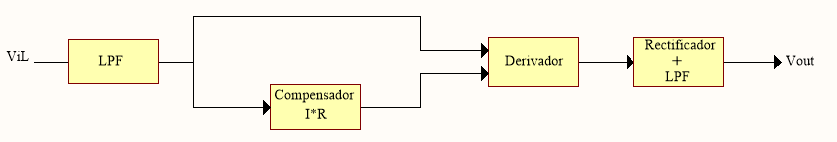
\includegraphics[scale=0.5]{Diagrama-Bloques-Estimador.png}
	\caption{Diagrama en bloques del estimador.}
	\label{fig:img_Diagrama-Bloques-Estimador.png}
\end{figure}

\section{An\'{a}lisis de la estimaci\'{o}n}

\noindent La ecuaci\'{o}n que gobierna la corriente en el electroim\'{a}n se puede calcular con las leyes de Kirchoff correspondientes al circuito que se ve en la figura \ref{fig:img_topologia-puenteH} y la expresión de la inductancia \ref{eq_inductancia_vs_y}.


\noindent Al resolver el circuito se obtiene:
\begin{equation} \label{eq_VbusCondicion}
	\pm V_{BUS}-\ L(Y_g)*\left|\frac{{di}_L}{dt}\right|-L_{\infty }*\left|\frac{{di}_L}{dt}\right|-R_L*I_L=0
\end{equation}


\noindent Se asume que:

\begin{equation} \label{eq_Derivadadi-dt}
	V_{BUS}>>i_L*R_L
\end{equation}
 
\noindent Se aproxima la derivada de la corriente como:

\begin{equation} \label{eq_derivadaAproximacion}
	\left|\frac{{di}_L}{dt}\right|\simeq \frac{V_{BUS}}{L(Y_g)+L_{\infty }}=\frac{V_{BUS}}{L_T(Y_g)}
\end{equation}

\noindent Según mediciones realizadas (ver tabla \ref{tab_mediciones}), se tienen los valores de $L_T(Y_g)$ correspondientes a cada posici\'{o}n. En base a ellos se hace una aproximaci\'{o}n lineal para obtener la expresi\'{o}n de la derivada de la ecuaci\'{o}n \ref{eq_di-dt_lineal}.

\noindent 

\begin{equation} \label{eq_di-dt_lineal}
{\left|\frac{{di}_L}{dt}\right|}_{Lineal}=\ 194690\ *\ Y[m]+676\ A/s
\end{equation}

\section{Modelo circuital del estimador de posici\'{o}n}

\noindent Para poder obtener $\left|\frac{{di}_L}{dt}\right|$ se utiliza un circuito derivador con un amplificador operacional como se observa en la figura  \ref{fig:img_Circuito-derivador}.

\begin{figure}[H]
	\centering
	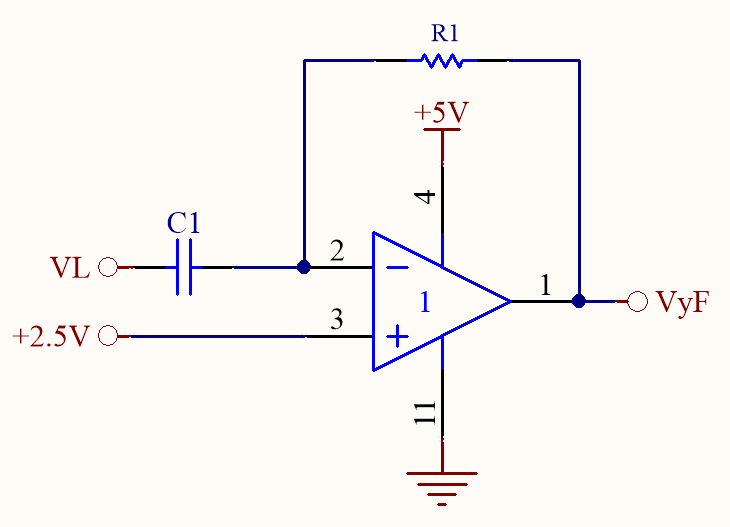
\includegraphics[scale=0.6]{Circuito-derivador.png}
	\caption{Circuito derivador.}
	\label{fig:img_Circuito-derivador}
\end{figure}

\noindent La salida del circuito $V_{yf}(t)$, ante una entrada $V_L$ es:

\begin{equation} \label{eq_vyf1}
	V_{yf}(t)\ =\ 2.5V\ -\ \frac{dV_L}{dt}*C_1*R_1
\end{equation}


\noindent Al considerar que $V_L=K_h*i_L$, con $K_h$ como la constante del sensor de efecto Hall, se obtiene: 

\begin{equation} \label{eq_vyf2}
	V_{yf}(t)\ =2.5\:V\ -\frac{di_L}{dt}*K_h*C_1*R_1
\end{equation}

\noindent $V_{yf}(t)$ tiene variaciones alrededor del set-point de $2.5\:V$. Por lo tanto, para evitar la saturaci\'{o}n del derivador se debe cumplir que:

\begin{equation} \label{eq_vyf3}
	\left|-\frac{di_L}{dt}*K_h*C_1*R_1\right|\ \le 2.5\:V
\end{equation}

\noindent Por lo tanto, con la ecuaci\'{o}n \ref{eq_derivadaAproximacion} y \ref{eq_vyf3}:

\begin{equation} \label{eq_condicionC1-R1}
	C_1*R_1\le\frac{2.5\ \:V\ *L_{min}}{V_{BUS}*K_h}
\end{equation}

\noindent Con $L_{min}= L(5\: mm) + L_{\infty}= 14.9\: mH$ se obtiene: 

\begin{equation} \label{eq_condicionC1-R1-2}
	C_1*R_1\le\ 29.1\ ms
\end{equation}

\noindent El derivador tiene como salida una onda pulsada, cuyo flanco superior  es proporcional a la pendiente de bajada de la corriente en el electroim\'{a}n, y el flanco inferior es proporcional a la pendiente de subida. 

\noindent Para los c\'{a}lculos se utiliz\'{o} $C_1*R_1= 25\: mS$, para dar un margen y evitar la saturaci\'{o}n del amplificador operacional.  

\noindent Con la ecuaci\'{o}n \ref{eq_di-dt_lineal} y \ref{eq_vyf2}, y con una variaci\'{o}n en torno a $2.5\:V$ se obtiene:


\begin{equation} \label{eq_Vyf-lineal}
	Vyf(Y_g)\ =\ |Kh*C_1*R_1*di/dt)|\ +2.5\:V=0.2595*Y_g+3.4\:V
\end{equation}

\noindent Se puede observar en la tabla \ref{tab_Vyf_vs_y} que, para los posibles valores en los que el electroim\'{a}n trabaja, el estimador posee un rango de salida ${\mathit{\Delta}{Vyf}_{Lineal}}(5\:mm-2\:mm)= 0.78\:V$.

\begin{table}[H]
	\begin{center}
		\begin{tabular}{| c | c |}
			\hline
			$Y_g[\:mm]$ & ${Vyf(Y_g)}_{Lineal} [\:V]$\\ \hline
			2 & 3.92 \\ \hline 
			3 & 4.18 \\ \hline 
			4 & 4.44 \\ \hline 
			5 & 4.7 \\ \hline 
		\end{tabular}
		\caption{$V_{yf}$ en función de la posición.}
		\label{tab_Vyf_vs_y}
	\end{center}
\end{table}

\section{Circuito del derivador compensado}

\noindent Puesto que los circuitos derivadores pueden presentar inestabilidad a alta frecuencia, es necesario compensarlos mediante el agregado de una resistencia en serie al capacitor, para que genere un cero en la transferencia de realimentaci\'{o}n (ecuación \ref{eq_Aw_2}), como se observa en la figura  \ref{fig:img_Circuito_derivador_compensado}.

\begin{figure}[H]
	\centering
	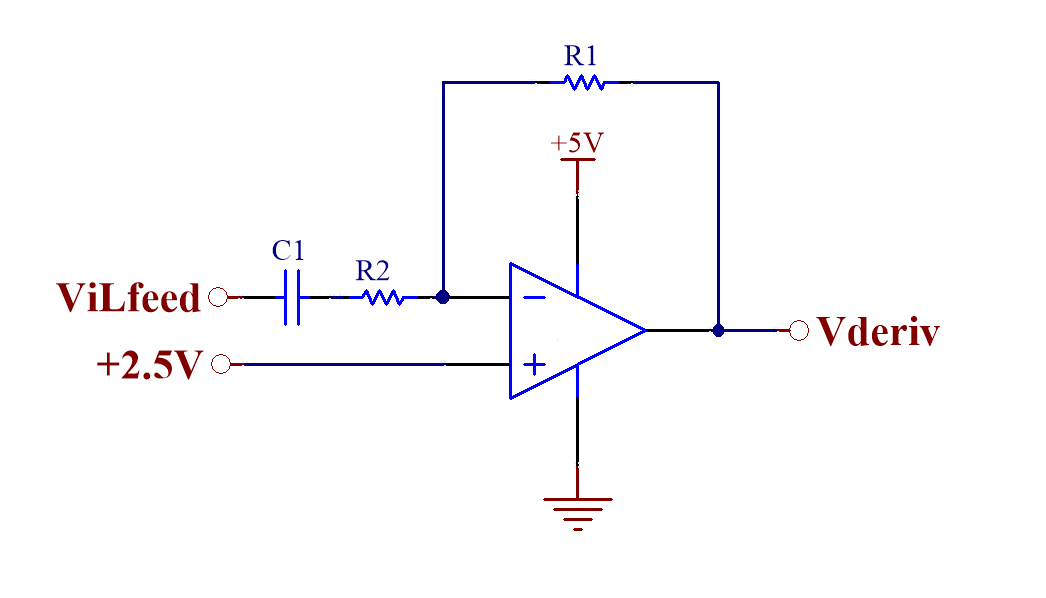
\includegraphics[scale=0.6]{Circuito-derivador- compensado.png}
	\caption{Circuito derivador compensado}
	\label{fig:img_Circuito_derivador_compensado}
\end{figure}

\noindent El operacional es internamente compensado, por lo que todos sus otros polos los tiene luego del cruce por $0\:dB$ de la ganancia. Para simplificar el an\'{a}lisis estos no se tienen en cuenta, ya que est\'{a}n fuera de la zona de inter\'{e}s.

\begin{equation} \label{eq_Aw_1}
	A(w)=\frac{1778279}{(\frac{s}{2\pi *20}+1)}
\end{equation} 

\begin{equation} \label{eq_Aw_2}
	\frac{1}{H(w)}=\frac{1+s*C_1*(R_1+R_2)}{1+s*C_1*R_2}\simeq \frac{1+s*C_1*R_1}{1+s*C_1*R_2}
\end{equation}

\noindent Para compensar el circuito se coloca un polo en $16 \:kHz$, que dá como resultado $R2=10\:\Omega$, $C1=1\:uF$ y $R1=25\: k\Omega$ y un margen de fase de $\phi =49.6{}^\circ $, como se puede observar en la figura \ref{fig:img_GH del derivador compensado}.

\begin{figure}[H]
	\centering
	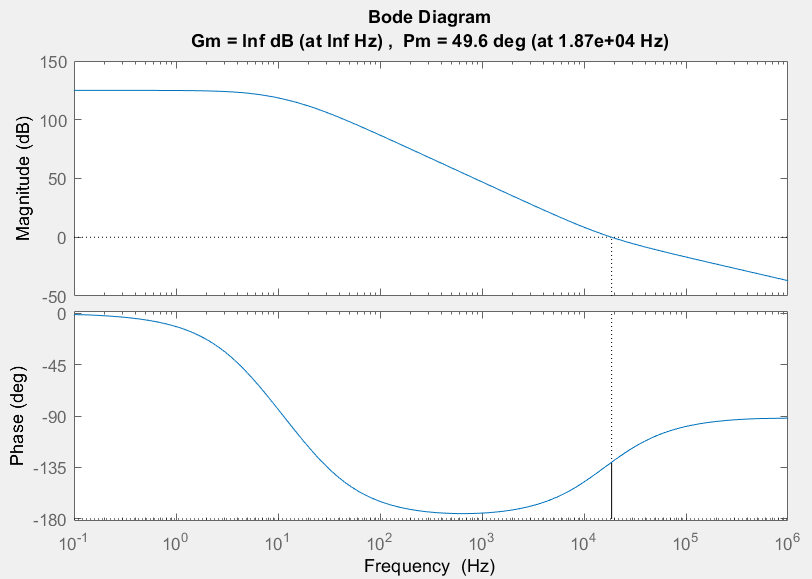
\includegraphics[scale=0.5]{GH-del-derivador-compensado.png}
	\caption{Transferencia a lazo abierto del derivador compensado.}
	\label{fig:img_GH del derivador compensado}
\end{figure}

\begin{figure}[H]
	\centering
	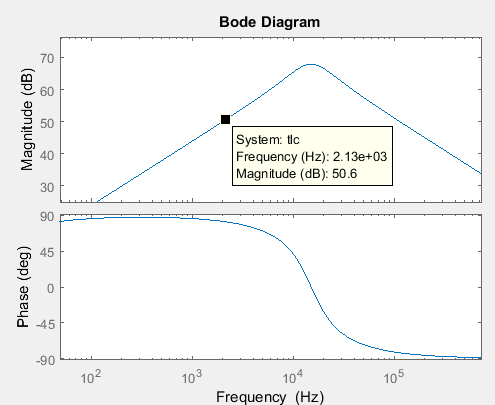
\includegraphics[scale=0.7]{Transferencia-de-lazo-cerrado.png}
	\caption{Transferencia de lazo cerrado.}
	\label{fig:img_Transferencia-de-lazo-cerrado}
\end{figure}

\noindent Como se observa en la figura \ref{fig:img_Transferencia-de-lazo-cerrado}, la transferencia de lazo cerrado (TLC) tiene un comportamiento derivativo en las frecuencias cercanas a $2 \:kHz$, como es deseado.

\noindent A continuaci\'{o}n se muestra la TLC del circuito derivador:
 
\begin{equation} \label{eq_Vyf-lineal}
	{TLC}_{derivador}=\frac{V_{yf}}{V_{iL}}=\frac{-0.025*s}{1+(\frac{2*0.473}{94,5\ krad/s})*s+(\frac{s}{94,5\ krad/s})^2}
\end{equation} 

\section{Dise\~{n}o del filtro pasa bajos}

\noindent Debido a que el derivador amplifica las se\~{n}ales de alta frecuencia es necesario agregar un filtro pasa bajos en su entrada. Como la se\~{n}al que ingresa al derivador es $V_{iL}$, que es una onda triangular de frecuencia fundamental de $2\:kHz$, se permite el paso de sus componentes hasta la 5º arm\'{o}nica. Para su implementaci\'{o}n se utiliza un filtro activo Butterworth de segundo orden, con una frecuencia de corte en $20\:kHz$. En la figura  \ref{fig:img_Filtro-para-la-entrada-del-derivador} se puede ver el filtro utilizado y en la figura \ref{fig:img_Respuesta-en-frecuencia-del-filtro-activo}, su respuesta en frecuencia.

\begin{figure}[H]
	\centering
	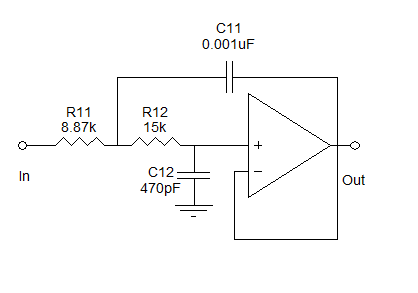
\includegraphics[scale=0.70]{Filtro-para-la-entrada-del-derivador.png}
	\caption{Filtro para la entrada del derivador.}
	\label{fig:img_Filtro-para-la-entrada-del-derivador}
\end{figure}

\begin{figure}[H]
	\centering
	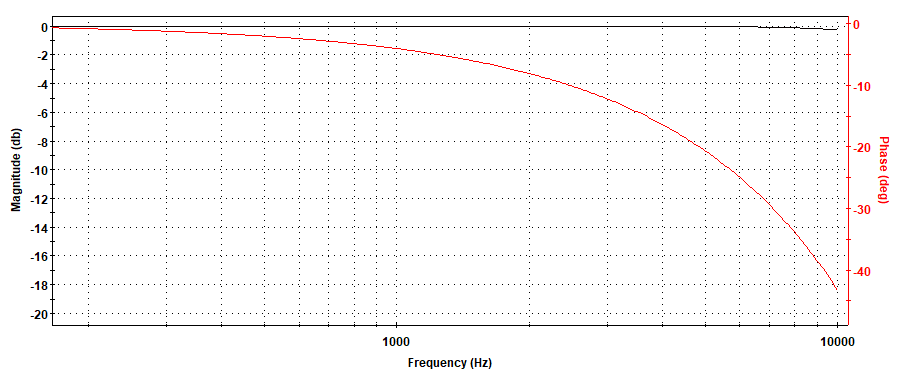
\includegraphics[scale=0.45]{Respuesta-en-frecuencia-del-filtro-activo.png}
	\caption{Respuesta en frecuencia del filtro activo.}
	\label{fig:img_Respuesta-en-frecuencia-del-filtro-activo}
\end{figure}

\section{Compensaci\'{o}n de resistencia interna}

\noindent Al circular corriente siempre en el mismo sentido por el electroim\'{a}n, se produce una ca\'{i}da de tensi\'{o}n casi constante en su resistencia interna. Esto provoca que no siempre est\'{e}n aplicados $\pm 24\:V$ al electroim\'{a}n sino que, durante el $T_{ON}$ se aplican $+24\:V-I*R$ y durante el $T_{OFF}$ se aplican $-24\:V-I*R$. Esto genera que las pendientes sean distintas.

\begin{equation} \label{eq_Vbus-didt-RL}
\pm V_{BUS}-L(y)*\left|\frac{{di}_L}{dt}\right|-L_{\infty }*\left|\frac{{di}_L}{dt}\right|-R_L*I_L=0
\end{equation}

\noindent Con  $R_L=0.2 \:\Omega$ y una corriente nominal  de $21\:A$:

\begin{equation} \label{eq_Vbus-didt-RL-2}
\pm V_{BUS}-R_L*I_L=\ \pm 24\:V-4.2\:V
\end{equation}

\noindent Para $V_{BUS}=24\:V$:

\begin{equation} \label{eq_Vbus-didt-RL-3}
	V_{BUS}-R_L*I_L=\ +24\:V-4.2\:V=\ 19.8\:V
\end{equation}

\noindent Para $V_{BUS}=-24\:V$

\begin{equation} \label{eq_Vbus-didt-RL-4}
	V_{BUS}-R_L*I_L=\ -24\:V-4.2\:V=\ 28.2\:V
\end{equation}

\noindent Por lo tanto, sobre el electroim\'{a}n se aplican dos tensiones distintas, en valor absoluto, durante la carga y descarga. Esto provoca que la rampa de corriente sea asim\'{e}trica.

\noindent Puesto que luego se utilizar\'{a} un rectificador de onda completa, se desea que la rectificaci\'{o}n de cada una de estas pendientes resulte en el mismo valor. En la figura \ref{fig:img_Forma-de-onda-luego-de-rectificar-sin-compensación-IR} se muestra el efecto luego de la rectificaci\'{o}n sin realizar ninguna compensaci\'{o}n:

\begin{figure}[H]
	\centering
	\includegraphics[scale=0.8]{Forma-de-onda-luego-de-rectificar-sin-compensación-IR.png}
	\caption{Forma de onda luego de rectificar sin compensación IR.}
	\label{fig:img_Forma-de-onda-luego-de-rectificar-sin-compensación-IR}
\end{figure}

\noindent Para corregir este problema, se varía set-point de la salida del derivador. Para lograrlo se debe cambiar la tensi\'{o}n en la entrada no inversora ($V_{bias}$) como se muestra en la figura \ref{fig:img_Esquema-circuital-del-derivador}. 

\begin{figure}[H]
	\centering
	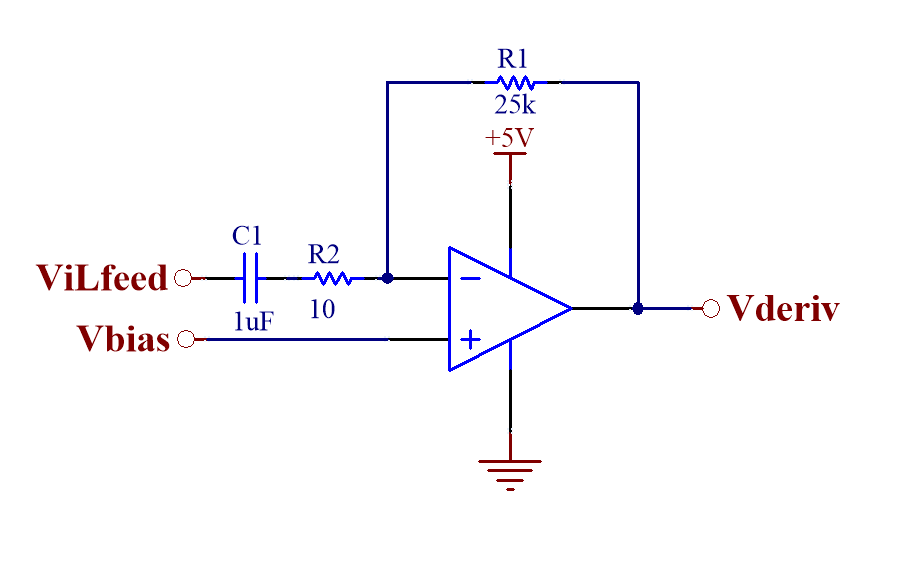
\includegraphics[scale=0.6]{Esquema-circuital-del-derivador.png}
	\caption{Esquema circuital del derivador con $V_{bias}$.}
	\label{fig:img_Esquema-circuital-del-derivador}
\end{figure}

\noindent Se tiene que la pendiente de bajada de la onda triangular, en m\'{o}dulo, es mayor que la de subida. Por lo tanto, al derivarla (con la inversi\'{o}n de signo), esta queda por encima del set-point, y la pendiente de subida, por debajo. Por ello, se debe compensar el set-point para que la forma de onda sea sim\'{e}trica alrededor de $2.5\:V$. 

\noindent Para la pendiente de bajada, la salida del derivador es:

\begin{equation} \label{eq_Vyf-Vbias}
	{Vyf}_{off}\ =\ V_{bias}+Kh\ *\ \tau *\frac{Vbus\ +\ Il*R}{L}\ 
\end{equation}

\noindent Para la pendiente de subida se tiene:

\begin{equation} \label{eq_Vyf-Vbias2}
	{Vyf}_{on}\ =\ V_{bias}\ -\ Kh\ *\ \tau *\frac{Vbus\ -\ Il*R}{L}
\end{equation}

\noindent Se desea que se cumpla:

\begin{equation} \label{eq_Vyf_Vbias3}
	{Vyf}_{off}\ -2.5\ \:V=\ 2.5\ V\ -{Vyf}_{on}
\end{equation}

\noindent Si se despeja $V_{bias}$ se llega a:

\begin{equation} \label{eq_Vyf-Vbias4}
	V_{bias}\ =2.5\ \:V -\ Kh\ *Il*\ \tau *\frac{\ R}{L}
\end{equation}

\noindent Se tiene $Kh = 53,3\:\frac{mV}{A},\; R = 0.2\:\Omega,\; \tau  = 25 \:ms$. En cuanto a la inductancia, se utiliza:  $L_T(4\:mm) = 16,44\:mHy$.

\noindent $V_{iL}$ es la tensi\'{o}n de salida del sensor de efecto Hall menos un set-point de $2.5\:V$. Sin embargo, debido al offset agregado al sensor para llevar su valor medio a $2.6\:V$, al restarle $2.5\:V$ no se produce una cancelaci\'{o}n completa sino que quedan $0.1\:V$ de error. Por ello, para implementar la ecuaci\'{o}n  \ref{eq_Vyf_Vbias3} se utiliza el circuito mostrado en la figura \ref{fig:img_Generación_de_Vbias}. Este circuito compensa la diferencia de pendientes, el error de $0.1\:V$ y genera $V_{bias}$ para ingresar al derivador.

\begin{figure}[H]
	\centering
	\includegraphics[scale=0.6]{Generación-de-Vbias.png}
	\caption{Generación de Vbias.}
	\label{fig:img_Generación_de_Vbias}
\end{figure}

\noindent A partir del circuito de la figura \ref{fig:img_Generación_de_Vbias} se obtiene:

\begin{equation} \label{eq_Vyf-Vbias3}
	V_{bias}\ =-\frac{R_4}{R_3}(K_hI_L+\ 0.1\:V)+V_{Ref_{bias}}(1+\frac{\ R_4}{R_3})*(\frac{R_1}{R_1+R_2})
\end{equation}

\noindent Para poder llegar a la expresi\'{o}n de la ecuaci\'{o}n \ref{eq_Vbus-didt-RL-2} se debe cumplir que:

\begin{enumerate}
	\item  $-\frac{R_4}{R_3}=-\ \tau *\frac{\ R}{L}=\ -0.304$  
	
	\item  $-\frac{R_4}{R_3}(\ 0.1V)+V_{Ref_{bias}}(1+\frac{\ R_4}{R_3})*(\frac{R_1}{R_1+R_2})\ =\ 2.5V$     
\end{enumerate}

\noindent Por lo tanto, al resolver la condici\'{o}n 1) se elige R4 = 304 $\mathit{\Omega}$ y se obtiene $R_3=1\ \:{k\mathit{\Omega}}$. Luego, al resolver la condici\'{o}n 2) con $V_{Ref_{bias}}=2.5\:V$ se elige $R_1=1k\:\mathit{\Omega}$ y se obtiene $R_{2\ }=291.8\:\mathit{\Omega}.$

\noindent En la figura \ref{fig:img_Formas_de_onda_obtenidas_en_la_simulación} se muestra como cambia la forma de onda.

\begin{figure}[H]
	\centering
	\includegraphics[scale=0.9]{Formas-de-onda-obtenidas-en-la-simulación.png}
	\caption{Formas de onda obtenidas en la simulación.}
	\label{fig:img_Formas_de_onda_obtenidas_en_la_simulación}
\end{figure}

\noindent La onda superior corresponde a la corriente en el electroim\'{a}n, la onda que se encuentra al medio, a la salida del derivador ${[V}_{bias}$$]$ y la inferior, a la onda rectificada con la correcci\'{o}n de la resistencia interna.

\section{Rectificador, Restador y Filtrado}

\subsection{Rectificador}

\begin{figure}[H]
	\centering
	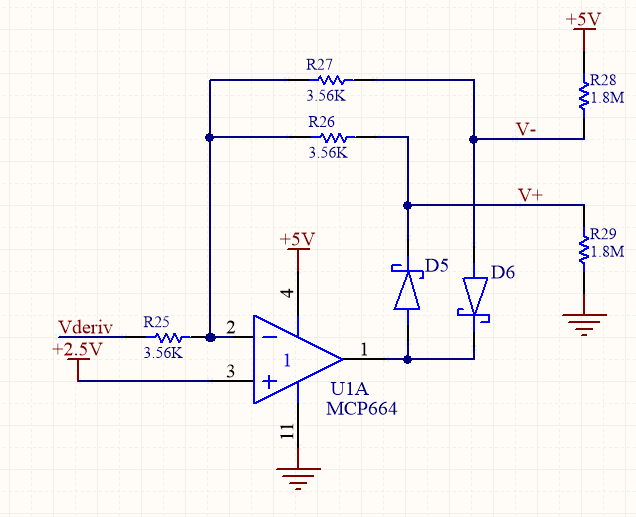
\includegraphics[scale=0.7]{Rectificador-y-restador.png}
	\caption{Rectificador.}
	\label{fig:img_Rectificador_y_restador}
\end{figure}

\noindent Para poder tener finalmente la estimaci\'{o}n de la posici\'{o}n, se debe rectificar la salida del derivador alrededor de $2.5\:V$. Esto se hace para hacer coincidir la pendiente positiva de la corriente triangular, con la pendiente negativa, y tener a la salida del estimador una se\~{n}al aproximadamente continua.

\noindent Para entender el funcionamiento de este rectificador, se comienza con el análisis de la etapa del primer amplificador operacional. Se parte de la suposici\'{o}n de que en un amplificador ideal, la tensi\'{o}n diferencial ($V_d$) es igual a cero. Por lo tanto, como la entrada no inversora est\'{a} fijada en $2.5\:V$, la misma tensi\'{o}n se encuentra en la entrada inversora.

\noindent Al analizar la corriente en la resistencia $R_{25}$ (se adpota el sentido positivo hacia la izquierda) en funci\'{o}n de $V_{deriv}$, resulta:

\begin{equation} \label{eq_corriente_r25}
	I_{R25}=\frac{2.5\:V\ -\ V_{deriv}}{R_{25}}
\end{equation}

\noindent En el caso de que $V_{deriv}$ $\mathrm{<}$ $2.5\:V$, la corriente ser\'{a} positiva. Esta misma corriente proviene desde la salida del operacional, a trav\'{e}s del diodo $D_5$ y por la resistencia $R_{26}$. Si se desprecia la tensi\'{o}n del diodo en directa, se obtiene que la salida del operacional es igual a V+, y esta es igual a:

\begin{equation} \label{eq_V+}
	V^+=I_{R25}*R_{26}+2.5\:V=\frac{2.5\:V-V_{deriv}\ }{R25}*R_{26}+2.5\:V\ 
\end{equation} 

Como $R_{25}=R_{26}$

\begin{equation} \label{eq_V+_2}
	V^+\ =\ 2.5\:V\ -\ V_{deriv}\ +2.5\:V\ =\ 5\:V\ -\ V_{deriv}\ 
\end{equation}

Además, dado que el diodo $D_6$ queda polarizado en inversa y la caída de tensión en $R_{26}$ es despreciable, se obtiene que $V^- = 2.5\:V$.

An\'{a}logamente, si $V_{deriv}$ $\mathrm{>}$ $2.5\:V$, se puede encontrar:

\begin{equation} \label{eq_V+_3}
	V^- =5\:V-V_{deriv} 
\end{equation}

\begin{equation} 
	V^+ = 2.5\:V
\end{equation}


\subsection{Restador}

\noindent Se utiliza un amplificador operacional en modo diferencial como restador. El circuito utilizado se observa en la figura \ref{fig:img_Restador} y se obtiene lo siguiente:

\noindent Cuando $V_{deriv}$ $\mathrm{<}$ $2.5\:V$:
\begin{equation*} 
	\begin{aligned}
		V_{estim}&=V^+-\ V^-\ +2.5\:V\\ 
		V_{estim}&=(5\:V -\ V_{deriv})-(2.5\: V)+2.5\:V\\
		V_{estim}&=5\: V\ -\ V_{deriv}\\ 
	\end{aligned}
\end{equation*}


\noindent Cuando $V_{deriv}$ $\mathrm{>}$ $2.5\:V$: 
\begin{equation*} 
	\begin{aligned}
		V_{estim}&=V^+-\ V^-+2.5V\\ 
		V_{estim}&=2.5V\ -\ (5V-\ V_{deriv})+\ 2.5V\\
		V_{estim}&=V_{deriv}\\
	\end{aligned}
\end{equation*}

\noindent Si se toma a $V_{deriv}$ como $V_{deriv}=\mathit{\Delta}V_{deriv}\ +\ 2,5\: V$, al reemplazar en los dos casos se obtiene:
\begin{equation} \label{eq_rest_3}
	Vestim=\ 2,5\ V\ +\ |\mathit{\Delta}V_{deriv}|
\end{equation}

\begin{figure}[H]
	\centering
	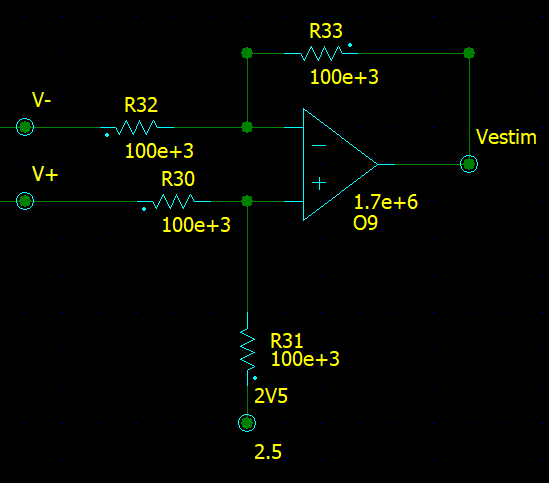
\includegraphics[scale=0.7]{Restador.png}
	\caption{Restador.}
	\label{fig:img_Restador}
\end{figure}

\subsection{Filtrado}

\noindent En el restador se implementa un filtrado adicional a la se\~{n}al de salida como se observa en la figura  \ref{fig:img_Esquema-circuital-del-restador-con-una-etapa-de-filtrado-en-159}. De esta \'{u}ltima etapa, si se considera $C_5=C_6=C\ $y $R_{33}=R_{31}=R$, se obtiene:



\begin{equation}
	V_{estim}=\frac{1}{1+S*C*R}*{(V}^+-V^-\ +\ 2.5\:V)
\end{equation}

\begin{equation} \label{eq_Vestim_1}
	V_{estim}=\frac{1}{1+S*C*R}*(2.5\: V\ +\ |\mathit{\Delta}V_{deriv}|)
\end{equation}

\begin{equation} \label{eq_Vestim_2}
	V_{estim} \approx \frac{1}{1+S*C*R}*\ |\mathit{\Delta}V_{deriv}|\ +2.5\:V
\end{equation}



\noindent Puesto que la salida $V_{estim}$ debe ser una continua, es importante eliminar cualquier posible ripple permitiendo solo el paso de continua. Por ello, se escogen los siguientes valores para los componentes:

\begin{enumerate}
	\item  $C=10\: nF$
	
	\item  $R=100\:\Omega$
	
	\item  $\frac{1}{2*\pi *C*R}=159.2\: Hz$
\end{enumerate}

\begin{figure}[H]
	\centering
	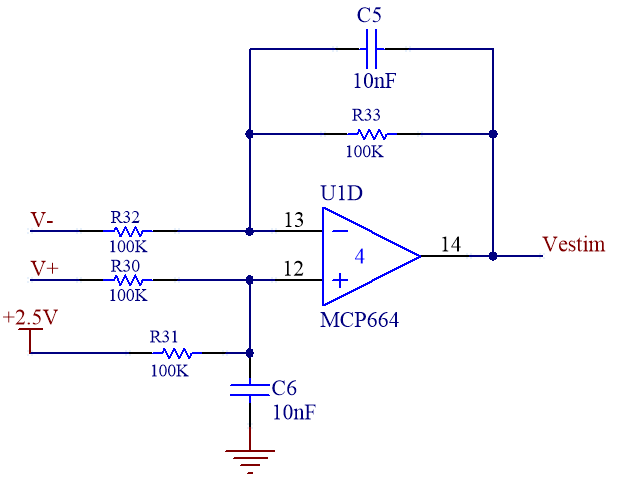
\includegraphics[scale=0.7]{Esquema-circuital-del-restador-con-una-etapa-de-filtrado-en-159.png}
	\caption{Esquema circuital del restador con una etapa de filtrado en $159.2\: Hz$.}
	\label{fig:img_Esquema-circuital-del-restador-con-una-etapa-de-filtrado-en-159}
\end{figure}

\section{Circuito completo}

\noindent En la figura \ref{fig:img_Circuito_estimador_de_posición_completo} se puede observar el circuito completo utilizado para la implementaci\'{o}n del rectificador, restador y filtrado.

\begin{figure}[H]
	\centering
	\includegraphics[scale=0.5]{Circuito-estimador-de-posición-completo.png}
	\caption{Circuito de rectificación, resta y filtrado.}
	\label{fig:img_Circuito_estimador_de_posición_completo}
\end{figure}

\section{Simulaci\'{o}n del estimador completo}

\noindent En la figura \ref{fig:img_Simulación_final_del_estimado} se pueden observar 3 formas de onda. La superior corresponde a la corriente del electroim\'{a}n, la del medio a la salida del derivador y la inferior a la salida $V_{estim}$. Con el uso de los cursores se midi\'{o} un ripple de $52.66\:mV $ en $V_{estim}$.

\begin{figure}[H]
	\centering
	\includegraphics[scale=0.6]{Simulación-final-del-estimador.png}
	\caption{Simulación final del estimador.}
	\label{fig:img_Simulación_final_del_estimado}
\end{figure}

\noindent En la figura \ref{tab_Resultados_de_simulación_del_estimador} se muestran valores medidos de Vestim en funci\'{o}n de la posici\'{o}n.

\begin{table}[H]
	\begin{center}
		\begin{tabular}{| c | c | c |}
			\hline
		$y [\:mm]$ & $L(y) [\:mH]$ & $V_{estim} [\:V]$ \\ \hline 
		2 & 22.64 & 3.86 \\ \hline 
		3 & 18.8 & 4.13 \\ \hline 
		4 & 16.44 & 4.36 \\ \hline 
		5 & 14.9 & 4.55 \\ \hline 
		\end{tabular}
		\caption{Resultados de simulación del estimador.}
		\label{tab_Resultados_de_simulación_del_estimador}
	\end{center}
\end{table}

\section{Transferencia final del estimador de posici\'{o}n:}

El funcionamiento del circuito estimador no es lineal.  Por lo tanto, para poder modelar una función transferencia, se deben tomar ciertas consideraciones. La parte del derivador es lineal, por lo que se puede modelar su transferencia como:
\begin{equation}
	V_{estim}=-0.025*\frac{dViL}{dt} 
\end{equation}

Esto significa que además de realizar la derivada, introduce una inversión de signo. De esta forma, una pendiente positiva a la entrada resulta en valores menores a $2.5\:V$ a la salida, mientras que una pendiente negativa produce una tensión mayor a $2.5\:V$.

Luego, el bloque rectificador y restador se encarga de calcular el valor absoluto de esta señal (en torno a los $2.5\:V$). Al considerar que la pendiente aumenta a medida que lo hace la distancia de separación, se puede concluir que el bloque estimador no produce inversión de signo. Por lo tanto, se debe considerar solamente la ganancia del derivador y el polo que introduce la etapa de restador. Finalmente, para poder obtener una estimación de la posición, se utiliza la expresión linealizada \ref{eq_di-dt_lineal} que relaciona $\frac{dI_{L}}{dt} = 194690 * Y_{g}$. Considerando que $\frac{dI_{L}}{dt} =\frac{dvi_{L}}{dt}*\frac{1}{0.0533}$, se obtiene que $\frac{dvi_{L}}{dt} = 0.0533*194690*Y_{g}$. 

Finalmente se obtiene que:

\begin{equation}
 V_{estim}=0.025*194690*0.0533 * \frac{Y_{g}}{1 + \frac{s}{1\:krad/seg}}=259.6*\frac{Y_{g}}{1 + \frac{s}{1\:krad/seg}}	
\end{equation}

\noindent Al considerar la etapa de filtrado de la entrada, que tiene dos polos en $2\pi *10\: \:{kHz}\ \simeq 60\: \:{krad/s}$ se obtiene:

\begin{equation} \label{eq_TLC_deriv_7}
	H_{estim}=\frac{V_{estim}}{Y_{g}[m]}=\frac{259.6}{(1+\frac{s}{1\: krad/s})*{(1+\frac{s}{60\: krad/s})}^2}
\end{equation}
